\documentclass[12pt]{article}

\usepackage{graphicx}
\usepackage{paralist}
\usepackage{amsfonts}
\usepackage{amsmath}
\usepackage{hhline}
\usepackage{booktabs}
\usepackage{multirow}
\usepackage{multicol}
\usepackage{url}
\usepackage{pdfpages}

\oddsidemargin -10mm
\evensidemargin -10mm
\textwidth 160mm
\textheight 200mm
\renewcommand\baselinestretch{1.0}

\pagestyle {plain}
\pagenumbering{arabic}

\newcounter{stepnum}

%% Comments

\usepackage{color}

\newif\ifcomments\commentstrue

\ifcomments
\newcommand{\authornote}[3]{\textcolor{#1}{[#3 ---#2]}}
\newcommand{\todo}[1]{\textcolor{red}{[TODO: #1]}}
\else
\newcommand{\authornote}[3]{}
\newcommand{\todo}[1]{}
\fi

\newcommand{\wss}[1]{\authornote{blue}{SS}{#1}}

\title{Assignment 4, Design Specification}
\author{SFWRENG 2AA4}

\begin{document}

\maketitle
This Module Interface Specification (MIS) document contains the modules necessary to implement the model and the view of the game \textit{2048}. At the start of the game, the player will see a 4x4 board containing 16 cells. Two random cells will contain either two \texttt{2} tiles, or one \texttt{2} tile and one \texttt{4} tile. The player can then move the tiles either up, down, left, or right, and the tiles slide over in that direction as far as they can go, unless they are blocked by the edge of the board, or another tile. If the tiles that slide together are the same, then they combine to create a single tile whose value is two times its original value. Therefore, all cells are either empty, or contain a tile whose value is $2^n$, where $n$ is a natural number not including $0$. For this implementation, the empty cells will be represented by a \texttt{0} tile. A visualization of the game board and an example of a move \texttt{right} is shown below:

% \begin{center}
%   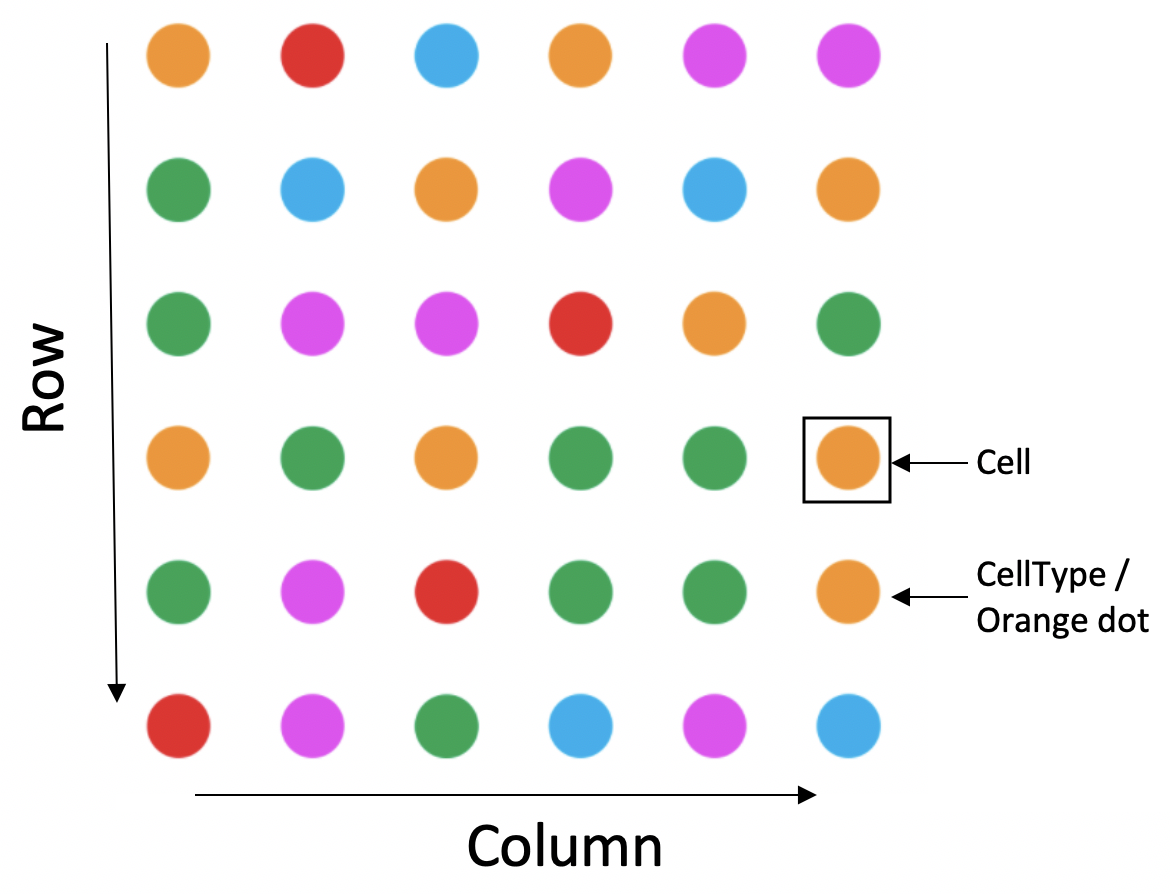
\includegraphics[width=0.7\textwidth]{naming.png}

%   The above board visualization is from https://play2048.co
% \end{center}

\newpage

\section{Overview of the design}

This design applies Model View Controller (MVC) design pattern, where \textit{BoardT} is the model module and \textit{View} is the view module. The module \textit{BoardT} stores the state of the game board and the status of the game, while the view module \textit{View} displays the current state of the game board and the overall game using text-based (ASCII) graphics. There is no controller module in this implementation.

\newpage

\subsection*{Likely Changes my design considers:}

\begin{itemize}
  \item Data structure used for storing the game board
  \item  
  \item 
  \item Change in game ending conditions to adjust the difficulty of the game.
\end{itemize}

\newpage

\section* {Board ADT Module}

\subsection*{Template Module}

BoardT

\subsection* {Uses}

None

\subsection* {Syntax}

\subsubsection* {Exported Types}

None

\subsubsection* {Exported Constant}

size = 4 \quad // Size of the board 4 x 4

\subsubsection* {Exported Access Programs}

\begin{tabular}{| l | l | l | l |}
\hline
\textbf{Routine name} & \textbf{In} & \textbf{Out} & \textbf{Exceptions}\\
\hline
BoardT & ~ & BoardT & \\
\hline
getBoard & ~ & seq of (seq of $\mathbb{N}$) & \\
\hline
getScore & ~ & $\mathbb{N}$ & \\
\hline
getHighScore & ~ & $\mathbb{N}$ & \\
\hline
emptyCells & ~ & set of (seq of $\mathbb{N}$) & \\
\hline
isGameWon & ~ & $\mathbb{B}$ & \\
\hline
isGameLost & ~ & $\mathbb{B}$ & \\
\hline
setBoard & seq of (seq of $\mathbb{N}$) & ~ & IllegalArgumentException\\
\hline
resetBoard  & ~ &  ~     & \\
\hline
isValidMoveRight  & ~ &  $\mathbb{B}$   & \\
\hline
isValidMoveLeft  &  ~  &  $\mathbb{B}$   & \\
\hline
isValidMoveUp  &  ~  &  $\mathbb{B}$   & \\
\hline
isValidMoveDown  &  ~  & $\mathbb{B}$ & \\
\hline
moveRight  & ~  &  ~     & \\
\hline
moveLeft  &  ~ &  ~     & \\
\hline
moveUp  &  ~  &  ~     & \\
\hline
moveDown  &  ~  &  ~     & \\
\hline
\end{tabular}

\subsection* {Semantics}

\subsubsection* {State Variables}

board: sequence [size, size] of $\mathbb{N}$ \\
score: $\mathbb{N}$ \\
highscore: $\mathbb{N}$ \\
empty: set of (sequence of $\mathbb{N}$) \\
win: $\mathbb{B}$ \\
lose: $\mathbb{B}$

\subsubsection* {State Invariant}

$0 \le |empty| \le 14$\\
$0 \le score \le highscore$

\subsubsection* {Assumptions}

\begin{itemize}
  \item The constructor BoardT is called for each object instance before any other access routine 
  is called for that object. 
  \item Assume there is a random function that generates a random value beteern 0 and 1.
  \item \textit{highscore} is a static variable.
  \item The seq of (seq of $\mathbb{N}$) provided as input for the \textit{setBoard} method will consist of correct numbers. This means that the numbers will be either $0$ to represent an empty cell, or $2^n$, where $n \ne 0$.
  \item The set of (sequence of $\mathbb{N}$) used to represent the state variable \textit{empty} will contain the coordinates for the empty cells of the game board. The sequence of $\mathbb{N}$ will only contain two numbers to represent the row and column of an empty cell. For example, \textit{empty} will be a set of $[row, column]$.
\end{itemize}

\subsubsection* {Access Routine Semantics}

BoardT():
\begin{itemize}
\item transition: \\
      board $:=$ 
      $\langle \begin{array}{c}
      \langle 0, 0, 0, 0 \rangle\\
      \langle 0, 0, 0, 0 \rangle\\
      \langle 0, 0, 0, 0 \rangle\\
      \langle 0, 0, 0, 0 \rangle\\
      \end{array} \rangle$ \\ 
      where two random empty cells are replaced with two \texttt{2} tiles or one \texttt{2} tile and one \texttt{4} tile.

      score, win, lose $=$ 0, False, False\\
      empty $:= \forall i, j : [0...size-1] | (board[i][j] = 0 \Rightarrow empty \cup \{\langle i, j \rangle\}$ $|$ $True \Rightarrow empty - \{\langle i, j \rangle\}$)
\item output: $out := \mathit{self}$
\item exception: None
\end{itemize}

\noindent getBoard():
\begin{itemize}
\item output: $out :=$ board
\item exception: None
\end{itemize}

\noindent getScore():
\begin{itemize}
\item output: $out :=$ score
\item exception: None
\end{itemize}

\noindent getHighScore():
\begin{itemize}
\item output: $out :=$ highscore
\item exception: None
\end{itemize}

\noindent emptyCells():
\begin{itemize}
\item output: $out :=$ empty
\item exception: None
\end{itemize}

\noindent isGameWon():
\begin{itemize}
\item output: $out :=$ win
\item exception: None
\end{itemize}

\noindent isGameLost():
\begin{itemize}
\item output: $out :=$ lose
\item exception: None
\end{itemize}

\noindent setBoard($b$):
\begin{itemize}
  \item transition: board $:= b$ 
  \item output: None
  \item exception: $exc :=$ (($\neg$ ($|b| = 4$) 
  $\Rightarrow$ IllegalArgumentException) $|$ 
  ($\forall(i : [0...size-1]$ $|$ $\neg (|b[i]| = 4) \Rightarrow$ IllegalArgumentException)))
\end{itemize}

\noindent resetBoard():
\begin{itemize}
\item transition:\\
      board $:=$ 
      $\langle \begin{array}{c}
      \langle 0, 0, 0, 0 \rangle\\
      \langle 0, 0, 0, 0 \rangle\\
      \langle 0, 0, 0, 0 \rangle\\
      \langle 0, 0, 0, 0 \rangle\\
      \end{array} \rangle$ \\ 
      where two random empty cells are replaced with two \texttt{2} tiles or one \texttt{2} tile and one \texttt{4} tile.

      score, win, lose $=$ 0, False, False\\
      empty $:= \forall i, j : [0...size-1] | (board[i][j] = 0 \Rightarrow empty \cup \{\langle i, j \rangle\}$ $|$ $True \Rightarrow empty - \{\langle i, j \rangle\}$)
\item output: None
\item exception: None
\end{itemize}

\noindent isValidMoveRight():
\begin{itemize}
\item output: $\forall i : [0...size-1]$ $(\forall j : [0...size-2]$ $|$ $(board[i][j] \ne 0 \land board[i][j+1]=0 \Rightarrow True$ $|$ $board[i][j] = board[i][j+1] \land board[i][j], board[i][j+1] \ne 0 \Rightarrow True$ $|$ $True \Rightarrow False))$
\item exception: None
\end{itemize}

\noindent isValidMoveLeft():
\begin{itemize}
\item output: $\forall i : [0...size-1]$ $(\forall j : [size-1...1]$ $|$ $(board[i][j] \ne 0 \land board[i][j-1]=0 \Rightarrow True$ $|$ $board[i][j] = board[i][j-1] \land board[i][j], board[i][j-1] \ne 0 \Rightarrow True$ $|$ $True \Rightarrow False))$
\item exception: None
\end{itemize}

\noindent isValidMoveUp():
\begin{itemize}
\item output: $\forall i : [size-1...1]$ $(\forall j : [0...size-1]$ $|$ $(board[i][j] \ne 0 \land board[i-1][j]=0 \Rightarrow True$ $|$ $board[i][j] = board[i-1][j] \land board[i][j], board[i-1][j] \ne 0 \Rightarrow True$ $|$ $True \Rightarrow False))$
\item exception: None
\end{itemize}

\noindent isValidMoveDown():
\begin{itemize}
\item output: $\forall i : [0...size-2]$ $(\forall j : [0...size-1]$ $|$ $(board[i][j] \ne 0 \land board[i+1][j]=0 \Rightarrow True$ $|$ $board[i][j] = board[i+1][j] \land board[i][j], board[i+1][j] \ne 0 \Rightarrow True$ $|$ $True \Rightarrow False))$
\item exception: None
\end{itemize}

\noindent moveRight():
\begin{itemize}
\item transition:\\ 
board $:=$ $\forall i : [0...size-1]$ $(\forall j : [0...size-2]$ $|$
\begin{table}[hbt!]
\centering
\begin{tabular}{|l|l|l|}
\cline{3-3}
\multicolumn{1}{l}{} &  & transition \\
\hline
\multicolumn{2}{|l|}{$board[i][j] \ne 0 \land board[i][j+1] = 0$} & board $:=$ shiftRight(i, j, board)\\
\hline
\shortstack{$(board[i][j], board[i][j+1] \ne 0$ \\$\land board[i][j] = board[i][j+1]$} & \shortstack{$2\times board[i][j] = 2048 \land$ \\ $\neg$(score $+ \: 2\times board[i][j] > $ highscore) } & \shortstack{board $:=$ combineRight(i, j, board)\\ score $:=$ score $+\: 2\times board[i][j]$\\ win $:=$ True}\\
\cline{2-3}
 & \shortstack{$2\times board[i][j] \ne 2048 \land$ \\ (score $+ \: 2\times board[i][j] > $ highscore) } & \shortstack{board $:=$ combineRight(i, j, board)\\ score $:=$ score $+\: 2\times board[i][j]$\\ highscore $:=$ score $+\: 2\times board[i][j]$}\\
\cline{2-3}
  & \shortstack{$2\times board[i][j] = 2048 \land$ \\ (score $+ \: 2\times board[i][j] > $ highscore) }  & \shortstack{board $:=$ combineRight(i, j, board)\\ score $:=$ score $+\: 2\times board[i][j]$\\ highscore $:=$ score $+\: 2\times board[i][j]$\\ win $:=$ True}\\
\cline{2-3}
  & True & \shortstack{board $:=$ combineRight(i, j, board)\\ score $:=$ score $+\: 2\times board[i][j]$}\\
\hline
\end{tabular}
\end{table}
\\
) // \textit{And also replaces one random empty cell (if it exists) with a \texttt{2} tile.}\\
lose $:= \neg$ (isValidMoveRight() $\lor$ isValidMoveLeft() $\lor$ isValidMoveUp $\lor$ isValidMoveDown()) $\Rightarrow True$\\
empty $:= \forall i, j : [0...size-1] | (board[i][j] = 0 \Rightarrow empty \cup \{\langle i, j \rangle\}$ $|$ $True \Rightarrow empty - \{\langle i, j \rangle\}$)
\item output: None
\item exception: None
\end{itemize}

\newpage

\noindent moveLeft():
\begin{itemize}
\item transition:\\ 
board $:=$ $\forall i : [0...size-1]$ $(\forall j : [size-1...1]$ $|$
\begin{table}[hbt!]
\centering
\begin{tabular}{|l|l|l|}
\cline{3-3}
\multicolumn{1}{l}{} &  & transition \\
\hline
\multicolumn{2}{|l|}{$board[i][j] \ne 0 \land board[i][j-1] = 0$} & board $:=$ shiftLeft(i, j, board)\\
\hline
\shortstack{$(board[i][j], board[i][j-1] \ne 0$ \\$\land board[i][j] = board[i][j-1]$} & \shortstack{$2\times board[i][j] = 2048 \land$ \\ $\neg$(score $+ \: 2\times board[i][j] > $ highscore) } & \shortstack{board $:=$ combineLeft(i, j, board)\\ score $:=$ score $+\: 2\times board[i][j]$\\ win $:=$ True}\\
\cline{2-3}
 & \shortstack{$2\times board[i][j] \ne 2048 \land$ \\ (score $+ \: 2\times board[i][j] > $ highscore) } & \shortstack{board $:=$ combineLeft(i, j, board)\\ score $:=$ score $+\: 2\times board[i][j]$\\ highscore $:=$ score $+\: 2\times board[i][j]$}\\
\cline{2-3}
  & \shortstack{$2\times board[i][j] = 2048 \land$ \\ (score $+ \: 2\times board[i][j] > $ highscore) }  & \shortstack{board $:=$ combineLeft(i, j, board)\\ score $:=$ score $+\: 2\times board[i][j]$\\ highscore $:=$ score $+\: 2\times board[i][j]$\\ win $:=$ True}\\
\cline{2-3}
  & True & \shortstack{board $:=$ combineLeft(i, j, board)\\ score $:=$ score $+\: 2\times board[i][j]$}\\
\hline
\end{tabular}
\end{table}
\\
) // \textit{And also replaces one random empty cell (if it exists) with a \texttt{2} tile.}\\
lose $:= \neg$ (isValidMoveRight() $\lor$ isValidMoveLeft() $\lor$ isValidMoveUp $\lor$ isValidMoveDown()) $\Rightarrow True$\\
empty $:= \forall i, j : [0...size-1] | (board[i][j] = 0 \Rightarrow empty \cup \{\langle i, j \rangle\}$ $|$ $True \Rightarrow empty - \{\langle i, j \rangle\}$)
\item output: None
\item exception: None
\end{itemize}

\newpage

\noindent moveUp():
\begin{itemize}
\item transition:\\ 
board $:=$ $\forall i : [size-1...1]$ $(\forall j : [0...size-1]$ $|$
\begin{table}[hbt!]
\centering
\begin{tabular}{|l|l|l|}
\cline{3-3}
\multicolumn{1}{l}{} &  & transition \\
\hline
\multicolumn{2}{|l|}{$board[i][j] \ne 0 \land board[i-1][j] = 0$} & board $:=$ shiftUp(i, j, board)\\
\hline
\shortstack{$(board[i][j], board[i-1][j] \ne 0$ \\$\land board[i][j] = board[i-1][j]$} & \shortstack{$2\times board[i][j] = 2048 \land$ \\ $\neg$(score $+ \: 2\times board[i][j] > $ highscore) } & \shortstack{board $:=$ combineUp(i, j, board)\\ score $:=$ score $+\: 2\times board[i][j]$\\ win $:=$ True}\\
\cline{2-3}
 & \shortstack{$2\times board[i][j] \ne 2048 \land$ \\ (score $+ \: 2\times board[i][j] > $ highscore) } & \shortstack{board $:=$ combineUp(i, j, board)\\ score $:=$ score $+\: 2\times board[i][j]$\\ highscore $:=$ score $+\: 2\times board[i][j]$}\\
\cline{2-3}
  & \shortstack{$2\times board[i][j] = 2048 \land$ \\ (score $+ \: 2\times board[i][j] > $ highscore) }  & \shortstack{board $:=$ combineUp(i, j, board)\\ score $:=$ score $+\: 2\times board[i][j]$\\ highscore $:=$ score $+\: 2\times board[i][j]$\\ win $:=$ True}\\
\cline{2-3}
  & True & \shortstack{board $:=$ combineUp(i, j, board)\\ score $:=$ score $+\: 2\times board[i][j]$}\\
\hline
\end{tabular}
\end{table}
\\
) // \textit{And also replaces one random empty cell (if it exists) with a \texttt{2} tile.}\\
lose $:= \neg$ (isValidMoveRight() $\lor$ isValidMoveLeft() $\lor$ isValidMoveUp $\lor$ isValidMoveDown()) $\Rightarrow True$\\
empty $:= \forall i, j : [0...size-1] | (board[i][j] = 0 \Rightarrow empty \cup \{\langle i, j \rangle\}$ $|$ $True \Rightarrow empty - \{\langle i, j \rangle\}$)
\item output: None
\item exception: None
\end{itemize}

\newpage

\noindent moveDown():
\begin{itemize}
\item transition:\\ 
board $:=$ $\forall i : [0...size-2]$ $(\forall j : [0...size-1]$ $|$
\begin{table}[hbt!]
\centering
\begin{tabular}{|l|l|l|}
\cline{3-3}
\multicolumn{1}{l}{} &  & transition \\
\hline
\multicolumn{2}{|l|}{$board[i][j] \ne 0 \land board[i+1][j] = 0$} & board $:=$ shiftDown(i, j, board)\\
\hline
\shortstack{$(board[i][j], board[i+1][j] \ne 0$ \\$\land board[i][j] = board[i+1][j]$} & \shortstack{$2\times board[i][j] = 2048 \land$ \\ $\neg$(score $+ \: 2\times board[i][j] > $ highscore) } & \shortstack{board $:=$ combineDown(i, j, board)\\ score $:=$ score $+\: 2\times board[i][j]$\\ win $:=$ True}\\
\cline{2-3}
 & \shortstack{$2\times board[i][j] \ne 2048 \land$ \\ (score $+ \: 2\times board[i][j] > $ highscore) } & \shortstack{board $:=$ combineDown(i, j, board)\\ score $:=$ score $+\: 2\times board[i][j]$\\ highscore $:=$ score $+\: 2\times board[i][j]$}\\
\cline{2-3}
  & \shortstack{$2\times board[i][j] = 2048 \land$ \\ (score $+ \: 2\times board[i][j] > $ highscore) }  & \shortstack{board $:=$ combineDown(i, j, board)\\ score $:=$ score $+\: 2\times board[i][j]$\\ highscore $:=$ score $+\: 2\times board[i][j]$\\ win $:=$ True}\\
\cline{2-3}
  & True & \shortstack{board $:=$ combineDown(i, j, board)\\ score $:=$ score $+\: 2\times board[i][j]$}\\
\hline
\end{tabular}
\end{table}
\\
) // \textit{And also replaces one random empty cell (if it exists) with a \texttt{2} tile.}\\
lose $:= \neg$ (isValidMoveRight() $\lor$ isValidMoveLeft() $\lor$ isValidMoveUp $\lor$ isValidMoveDown()) $\Rightarrow True$\\
empty $:= \forall i, j : [0...size-1] | (board[i][j] = 0 \Rightarrow empty \cup \{\langle i, j \rangle\}$ $|$ $True \Rightarrow empty - \{\langle i, j \rangle\}$)
\item output: None
\item exception: None
\end{itemize}

\subsubsection* {Local Functions}

shiftRight: $\mathbb{N} \times \mathbb{N} \times$ seq of (seq of $\mathbb{N}$) $\rightarrow$ seq of (seq of $\mathbb{N}$) 

\medskip

\noindent shiftRight($i, j, board$) $\equiv$ $\forall x : [j+1...0]$ $|$ $(x = 0 \Rightarrow board[i][x] = 0$ $|$ $True \Rightarrow board[i][x] = board[i][x-1])$

\bigskip
\bigskip

\noindent combineRight: $\mathbb{N} \times \mathbb{N} \times$ seq of (seq of $\mathbb{N}$) $\rightarrow$ seq of (seq of $\mathbb{N}$)

\medskip

\noindent combineRight($i, j, board$) $\equiv$ $\forall x : [j+1...0]$ $|$ $(x = j+1 \Rightarrow board[i][x] = 2 \times board[i][x]$ $|$ $x = 0 \Rightarrow board[i][x] = 0$ $|$ $True \Rightarrow board[i][x] = board[i][x-1])$

\bigskip
\bigskip

\noindent shiftLeft: $\mathbb{N} \times \mathbb{N} \times$ seq of (seq of $\mathbb{N}$) $\rightarrow$ seq of (seq of $\mathbb{N}$) 

\medskip

\noindent shiftLeft($i, j, board$) $\equiv$ $\forall x : [j-1...size-1]$ $|$ $(x = 0 \Rightarrow board[i][x] = 0$ $|$ $True \Rightarrow board[i][x] = board[i][x+1])$

\bigskip
\bigskip

\noindent combineLeft: $\mathbb{N} \times \mathbb{N} \times$ seq of (seq of $\mathbb{N}$) $\rightarrow$ seq of (seq of $\mathbb{N}$)

\medskip

\noindent combineLeft($i, j, board$) $\equiv$ $\forall x : [j-1...size-1]$ $|$ $(x = j-1 \Rightarrow board[i][x] = 2 \times board[i][x]$ $|$ $x = size-1 \Rightarrow board[i][x] = 0$ $|$ $True \Rightarrow board[i][x] = board[i][x+1])$

\bigskip
\bigskip

\noindent shiftUp: $\mathbb{N} \times \mathbb{N} \times$ seq of (seq of $\mathbb{N}$) $\rightarrow$ seq of (seq of $\mathbb{N}$) 

\medskip

\noindent shiftUp($i, j, board$) $\equiv$ $\forall x : [i-1...size-1]$ $|$ $(x = size-1 \Rightarrow board[x][j] = 0$ $|$ $True \Rightarrow board[x][j] = board[x+1][j])$

\bigskip
\bigskip

\noindent combineUp: $\mathbb{N} \times \mathbb{N} \times$ seq of (seq of $\mathbb{N}$) $\rightarrow$ seq of (seq of $\mathbb{N}$)

\medskip

\noindent combineUp($i, j, board$) $\equiv$ $\forall x : [i-1...size-1]$ $|$ $(x = i-1 \Rightarrow board[x][j] = 2 \times board[x][j]$ $|$ $x = size-1 \Rightarrow board[x][j] = 0$ $|$ $True \Rightarrow board[x][j] = board[x+1][j])$

\bigskip
\bigskip

\noindent shiftDown: $\mathbb{N} \times \mathbb{N} \times$ seq of (seq of $\mathbb{N}$) $\rightarrow$ seq of (seq of $\mathbb{N}$) 

\medskip

\noindent shiftDown($i, j, board$) $\equiv$ $\forall x : [i+1...0]$ $|$ $(x = 0 \Rightarrow board[x][j] = 0$ $|$ $True \Rightarrow board[x][j] = board[x-1][j])$

\bigskip
\bigskip

\noindent combineDown: $\mathbb{N} \times \mathbb{N} \times$ seq of (seq of $\mathbb{N}$) $\rightarrow$ seq of (seq of $\mathbb{N}$)

\medskip

\noindent combineDown($i, j, board$) $\equiv$ $\forall x : [i+1...0]$ $|$ $(x = i+1 \Rightarrow board[x][j] = 2 \times board[x][j]$ $|$ $x = 0 \Rightarrow board[x][j] = 0$ $|$ $True \Rightarrow board[x][j] = board[x-1][j])$

\bigskip
\bigskip


\newpage

\section* {View Module (Abstract Object)}

\subsection* {Module}

View

\subsection* {Uses}

BoardT

\subsection* {Syntax}

\subsubsection* {Exported Types}

None

\subsubsection* {Exported Constants}

None

\subsubsection* {Exported Access Programs}

\begin{tabular}{| l | l | l | p{6cm} |}
\hline
\textbf{Routine name} & \textbf{In} & \textbf{Out} & \textbf{Exceptions}\\
\hline
printWelcomeMessage & ~ & ~ &  \\
\hline
printBoard & BoardT & ~ & \\
\hline
printMovePrompt & ~ & ~ & \\
\hline
printScore & BoardT & ~ & \\
\hline
printHighScore & BoardT & ~ & \\
\hline
printLosingMessage & ~ & ~ & \\
\hline
printWinningMessage & ~ & ~ & \\
\hline
printFarewellMessage & ~ & ~ & \\
\hline
\end{tabular}

\subsection* {Semantics}

\subsection*{Environment Variables}

terminal: displays the game, messages, and prompts to the player

\subsubsection* {State Variables}

None

\subsubsection* {State Invariant}

None

\subsubsection* {Access Routine Semantics}

\noindent printWelcomeMessage():
\begin{itemize}
  \item transition: terminal $:=$ Displays a welcome message when the player begins the game for the first time.
\end{itemize}

\noindent printBoard():
\begin{itemize}
\item transition: terminal $:=$ Displays the game board. The cells can be accessed by using the $getBoard$ method from $BoardT$. The board is displayed as a 4x4 matrix, so each row of cells is on a separate line. The board[x][y] is displayed so that x increases as you go right across the screen, and y increases as you go down the screen.
\end{itemize}

\noindent printMovePrompt():
\begin{itemize}
\item transition: terminal $:=$ Displays a prompt asking the player to select which direction they want to move the tiles.
\end{itemize}

\noindent printScore($b$):
\begin{itemize}
\item transition: terminal $:=$ Displays the current score of the game, which can be accessed by using the $getScore$ method from $BoardT$.
\end{itemize}

\noindent printHighScore($b$):
\begin{itemize}
\item transition: terminal $:=$ Displays the best/highest score of the game, which can be accessed by using the $getHighScore$ method from $BoardT$.
\end{itemize}

\noindent printLosingMessage():
\begin{itemize}
\item transition: terminal $:=$ Displays a message telling the player they lost, then displays a prompt asking the player if they would like to try again or exit the game.
\end{itemize}

\noindent printWinningMessage():
\begin{itemize}
\item transition: terminal $:=$ Displays a message telling the player they won, then displays a prompt asking the player if they would like to continue the current game, start a new game, or exit the game.
\end{itemize}

\noindent printFarewellMessage():
\begin{itemize}
\item transition: terminal $:=$ Displays a farewell message after the player decides to exit the game.
\end{itemize}

\newpage

\section*{Critique of Design}

\begin{itemize}
  \item I choose to specify BoardT module as ADT over abstract object, because It is more convenient to create a new instance of the board after the 
        user choose to restart a game.
  \item The controller and view modules are specified as a single abstract object because these modules are shared resources and only one instance is required
        to control the action during runtime. Thus, any conflicting or unexpected state changes can be avoided.
  \item The $getCell()$ method in $BoardT$ module is not essential. I added this method 
        is mainly for the high usability for the view module to display the status of the game.
  \item EndCondition interface provides some to generality to this design when comes to solving the problem of switching objective.
        I choose it to be an interface instead of a generic module because, in Java, you can only implement multiple interfaces but only one inheritance. Also, it 
        is easier to apply the strategy design pattern.
  \item The $gameStatus$ method in $EndByMoves$ and $EndByTime$ violates the principle of minimality. I design this module in this way is to ensure
        there is no delay or friction with the model module since the method updates the status of the game after each move made by the user during runtime.
  \item The two constructors in BoardT improve the flexibilty of the module. The user can choose to play with a board 
        initialized with randomly generated dots or a board that is customized or pre-defined. Also, from a testing perspective, methods can be 
        easily tested if the board is pre-defined compared to a randomly generated board.
  \item The test cases are designed to validate the correctness of the program based on the requirement and reveal errors
        or unusual behavior during program execution, every access routine has at least one test case. One exception is
        made for $replaceEliminated$ method in BoardT because the $replaceEliminated$ method adds a random dot to the board, 
        there are no efficient ways to test the correctness of adding a randomly generated cell.
  \item In $BoardT$, the result of $remove$ and $replaceEliminated$ method is tested using $getMessage$ method. These methods do
        not output anything and $getMessage$ method stores the information of the scoreboard, it updates after each successful dot removal.
  \item Did not build any test cases for testing the controller module since the implementation of the controller's access methods uses 
        methods from the model and view. The test cases for the model are in $TestBoardT.java$
  \item Using MVC also makes my design maintainable and reduces risk when making changes. MVC decomposes into three 
        component based on the separation of concerns where the model component encapsulates the internal 
        data and status of the game, the view displays the state of the game, and the controller handles
        the input actions to execute related actions to respond to events.
  \item My design achieves high cohesion and low coupling by applying MVC. MVC keeps high cohesion since
        it groups related functionalities within each module. The deisgn is also low coupling because
        the modules (model, view, controller) are mostly independent of each other. So a change in one of the
        modules does not heavily impact the other.
  \item A strategy design pattern provides convenience and flexibility when comes to design for change. It is easier to switch
        between different algorithms during runtime through polymorphism with the Strategy pattern. In addition, it increases
        maintainability and readability in a way that the concerns are separated into classes instead of using
        conditional statements to switch strategy in runtime.
  \item I found using the Singleton design pattern is better than using static methods for abstract objects. During the developing process, using 
        static methods and variables usually cause some warnings about the method or variables to need to be accessed statically. Using singleton
        pattern eliminates all these problems, making a smoother development.
  
\end{itemize}

\noindent Q1: Draw a UML diagram for the modules in A3.

\noindent Q2: Draw a control flow graph for the convex hull algorithm

%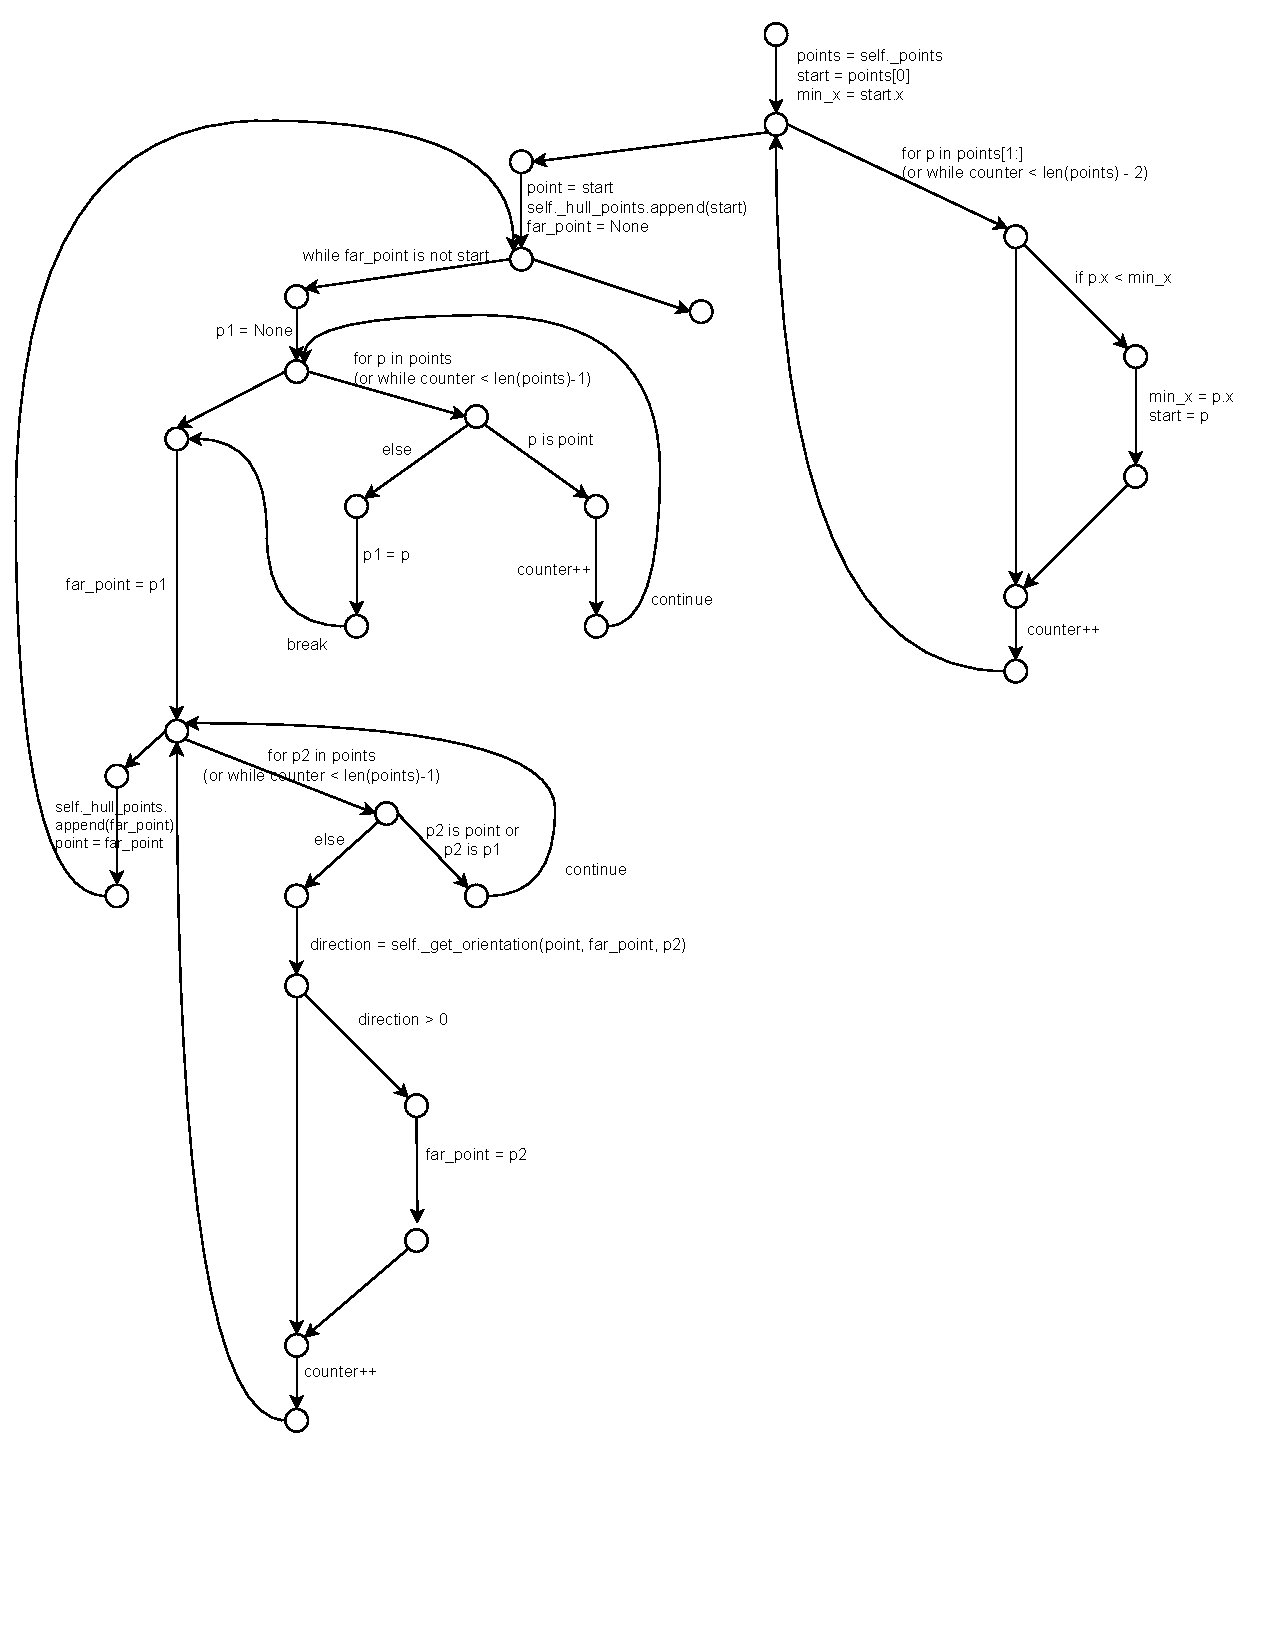
\includepdf[pages=-]{ControlFlow}
% \begin{center}
%   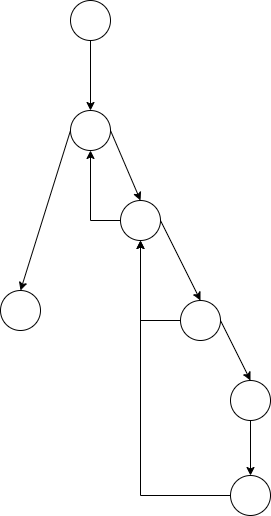
\includegraphics[width=0.3\textwidth]{Control_Flow_Graph.png} \\
%   The control flow graph is constructed using https://app.diagrams.net/
% \end{center}

\end {document}